% cd ..\..\Users\NikitaSkybytskyi\Desktop\c3s1\complex-analysis
\documentclass[a4paper, 12pt]{article}
\usepackage[utf8]{inputenc}
\usepackage[english, ukrainian]{babel}

\usepackage{amsmath, amssymb}
\usepackage{multicol}
\usepackage{graphicx}
\usepackage{float}
\usepackage{multicol}

\usepackage{amsthm}
\newtheorem{theorem}{Теорема}[subsection]
\newtheorem*{theorem*}{Теорема}
\newtheorem{lemma}{Лема}[subsection]
\newtheorem*{lemma*}{Лема}
\newtheorem*{remark*}{Зауваження}
\theoremstyle{definition}
\newtheorem*{definition}{Визначення}
\newtheorem{problem}{Задача}[section]
\newtheorem*{solution}{Розв'язок}
\newtheorem{example}{Приклад}
\newtheorem*{example*}{Приклад}
\newtheorem*{hint}{Вказівка}

\newcommand{\Max}{\displaystyle\max\limits}
\newcommand{\Sum}{\displaystyle\sum\limits}
\newcommand{\Int}{\displaystyle\int\limits}
\newcommand{\Lim}{\displaystyle\lim\limits}

\newcommand{\RR}{\mathbb{R}}
\newcommand{\ZZ}{\mathbb{Z}}

\newcommand*\diff{\mathop{}\!\mathrm{d}}
\newcommand*\Diff[1]{\mathop{}\!\mathrm{d^#1}}

\DeclareMathOperator{\Real}{Re}
\DeclareMathOperator{\Imag}{Im}

\DeclareMathOperator{\Arg}{Arg}

\DeclareMathOperator{\Ln}{Ln}

\DeclareMathOperator{\Arctan}{Arctan}
\DeclareMathOperator{\Arcsin}{Arcsin}
\DeclareMathOperator{\Arccos}{Arccos}
\DeclareMathOperator{\Arccosh}{Arccosh}
\DeclareMathOperator{\Arctanh}{Arctanh}

\DeclareMathOperator{\arcsinh}{arcsinh}
\DeclareMathOperator{\arccosh}{arccosh}
\DeclareMathOperator{\arctanh}{arctanh}
\DeclareMathOperator{\arccoth}{arccoth}

\newcommand{\varLimsup}{\varlimsup\limits}

\makeatletter
\newcommand\xLeftrightarrow[2][]{%
  \ext@arrow 9999{\longLeftrightarrowfill@}{#1}{#2}}
\newcommand\longLeftrightarrowfill@{%
  \arrowfill@\Leftarrow\relbar\Rightarrow}
\makeatother

\renewcommand{\epsilon}{\varepsilon}
\renewcommand{\phi}{\varphi}

\allowdisplaybreaks
\setlength\parindent{0pt}
\numberwithin{equation}{subsection}

\usepackage{xcolor}
\usepackage{hyperref}
\hypersetup{unicode=true,colorlinks=true,linktoc=all,linkcolor=red}

\numberwithin{equation}{section}% reset equation counter for sections
\numberwithin{equation}{subsection}
% Omit `.0` in equation numbers for non-existent subsections.
\renewcommand*{\theequation}{%
  \ifnum\value{subsection}=0 %
    \thesection
  \else
    \thesubsection
  \fi
  .\arabic{equation}%
}


\lhead{Бази даних, 2018}

\begin{document}

\section{Реляційна алгебра}
    \subsection{Теорія}
        \subsubsection{Лекція}
У кожній алгебрі є \textit{носій} (множина елементів з якими ми оперуємо) та \textit{сигнатура} (множина операцій). Сигнатура складається з восьми операцій, аргументами і результатами яких є реляційні відношення. Нехай $A$ і $B$ -- сумісні відношення, тобто відношення з однаковими атрибутами. Тоді для них визначені наступні \textit{операції}: $A\cup B$ (\textbf{об'єднання}) (для зручності будемо писати \verb|A UNION B||), $A\cap B$ (\textbf{перетин}) (для зручності будемо писати \verb|A INTERSECT B|) і $A\setminus B$ (\textbf{різниця}). \\

\textbf{Вибірка} $A[\langle\text{умова}\rangle]$ -- сумісне з $A$ відношення, тіло якого складається з тих елементів $A$ які задовольняють умову. \textbf{Проекція} $A\{\langle\text{список атрибутів}\rangle\}$ -- відношення, заголовок якого складається із вказаного списку, а тіло складається із кортежів тіла $A$ з яких вилучені елементи що відповідають атрибутам що не входять у список. Якщо в результаті проекції утворюють повторювані кортежі, то залишаємо по одному екземпляру кожного з них. \\ 

Нехай $A$ і $B$ -- відношення, що не містять однойменних атрибутів, тоді (декартовим) \textbf{добутком} $A\times B$ називається відношення, заголовок якого містить всі атрибути $A$ та всі атрибути $B$, а тіло є декартовим добутком тіл $A$ і $B$. Якщо заголовки $A$ і $B$ містять однойменні атрибути, то є два виходи: перший полягає у додаванні ідентифікаторів $\langle\text{ім'я відношення}\rangle.\langle\text{ім'я атрибута}\rangle$, а другий у застосуванні операції $A \texttt{ RENAME } x \texttt{ AS } y$.\\

Нехай $A$ і $B$ -- відношення, що не містять однойменних атрибутів, тоді їх \textbf{з'єднанням} називається $A[\langle\text{умова}\rangle]B$, заголовок якого складається з усіх атрибутів $A$ та усіх атрибутів $B$, а тіло буде складатися з усіх можливих пар кортежів $A$ і $B$ які задовольняють умову. Є природне з'єднання для відношень, заголовки яких мають спільні атрибути, тоді природнім з'єднанням називається відношення $A*B$, а тіло складається з тих зчеплень кортежів тіл $A$ і $B$ для яких значення спільних атрибутів однакові.\\

Останньою операцією є тернарна операція \textbf{ділення}. Нехай є відношення $A$ з атрибутами $x_1, \ldots, x_n$, відношення $B$ з атрибутами $y_1, \ldots, y_m$ і відношення $C$ з атрибутами $x_{i_1}, \ldots, x_{i_k}, y_{j_1},\ldots, y_{j_l}, z_1, \ldots, z_t$ (як правило, $x_{i_1}, \ldots, x_{i_k}$ -- ключі $A$ ... ). Результатом ділення називається відношення $A \div B \text{ per } C$ (для зручності будемо писати \verb|A DIV B PER C|) яке сумісне з $A$ і містить ті кортежі тіла $A$, які з'єднані з \textbf{усіма} кортежами $B$ через зв'язуюче відношення $C$.\\

Пріоритети операцій: вибірка, проекція $\succ$ решта, зліва направо. Пріоритети можна змінювати круглими дужками. \\

Насправді повний набір операцій складається з об'єднання, різниці, проекція, вибірки та декартового добутку, решта -- надлишкові. \\

Допускаються також прості функції, як-то \verb|count(·)|, \verb|sum(·)|, \verb|average(·)|.

\subsubsection{Моя власна інтерпретація}
Тимчасово відсутня, буде коли у мене буде на це час і бажання.

    \subsection{Практика}
        \subsubsection{Приклади з лекції}
Розглянемо кілька прикладів запитів до бази \ref{fig:supply}. Для зручності запити відформатовані за рівнем вкладеності:
\begin{enumerate}
    \item Імена лондонських постачальників зі статусом більше 10.
    \begin{verbatim}
    provider[
        city = 'London' 
        AND 
        status > 10
    ] {provider.name}.
    \end{verbatim}
    
    \item Номери деталей, які постачаються лондонськими постачальниками.
    \begin{verbatim}
    (
        provider[city = 'Lomdon]
        *
        supply
    ) {part_id}.
    \end{verbatim}
    
    \item Назви деталей, які постачаються Лондонськими постачальниками.
    \begin{verbatim}
    (
        (
            provider[city = 'London']
            *
            supply
        ) {part_id}
        *
        part
    ) {part.name}.
    \end{verbatim}
    
    \item Назви деталей, які не постачаються Лондонськими постачальниками.
    \begin{verbatim}
    (
        (
            part{part_id} 
            \ 
            (
                provider[city = 'London']
                * 
                supply
            ) {part_id}
        )
        * 
        part
    ) {part.name}.
    \end{verbatim}
    
    \item Назви деталей, які постачаються лише лондонськими постачальниками.
    \begin{verbatim}
    (
        (
            part{part_id}
            \ 
            (
                provider[city != 'London']
                *
                supply
            ) {part_id}
        )
        *
        part
    ) {part.name}.
    \end{verbatim}
    
    \item Імена постачальників, яка постачають всі деталі.
    \begin{verbatim}
    (
        provider{provider_id}
        DIV
        part{part_id}
        PER
        supply
    )
    *
    provider{provider.name}.
    \end{verbatim}
    або
    \begin{verbatim}
    (
        provider
        DIV
        part
        PER
        supply
    ) {provider.name}.
    \end{verbatim}
    
    \item Назви деталей, які постачаються всіма лондонськими постачальниками.
    \begin{verbatim}
    (
        part
        DIV
        provider[city = 'London']
        PER 
        supply
    ) {part.name}.
    \end{verbatim}
    
    \item Імена постачальників, які постачають червоні деталі в усі лондонські проекти.
    \begin{verbatim}
    (
        provider
        DIV
        project[city = 'London']
        PER
        (
            supply
            *
            part[color = 'red']
        )
    ) {provider.name}.
    \end{verbatim}
    
    \item Імена постачальників, які постачають лише ті деталі, які постачає Джон.
    \begin{verbatim}
    (
        (
            provider{provider_id}
            \ 
            (
                supply
                *
                (
                    part{part_id} 
                    \ 
                    (
                        (
                            provider[name = 'John']
                            *
                            supply
                        ) {part_id} 
                    )
                )
            ) {provider_id}
        )
        * 
        provider
    ) {provider.name}.
    \end{verbatim}
    
    \item Міста з яких всі постачальники постачають червоні деталі.
    \begin{verbatim}
    provider{city} 
    \ 
    (
        (
            provider{provider_id}
            \ 
            (
                part[color = 'red']
                *
                supply
            ) {provider_id}
        )
        *
        provider
    ) {provider.city}.
    \end{verbatim}
    
    \item Номери постачальників, які постачають певну деталь постачають в усі проекти
    \begin{verbatim}
    (
        supply{provider_id, part_id} 
        DIV
        project
        PER
        supply
    ) {provider_id}.
    \end{verbatim}
\end{enumerate}

\subsubsection{Запити на к/р (без розв'язків)}

\begin{card}
    \item Знайти прізвища та телефони лекторів з науковим ступенем доктора, які проводять другу пару у середу. 
    \item Знайти коди та курси груп, у яких Іванчук не проводить заняття у середу.
    \item Визначити аудиторії в яких займаються тільки групи 1-го курсу факультету кібернетики.
\end{card}

\begin{card}
    \item Знайти прізвища та організації лекторів, які читають с\textbackslashк (тип) на 3-ому курсі.
    \item Знайти назви предметів, які Іванчук не читає в аудиторії 205.
    \item Знайти прізвища лекторів з наук. ступенем доктора, які проводять заняття принаймні у всі ті дні, що і Іванчук. 
\end{card}

\begin{card}
    \item Знайти назви предметів та форми їх контролю, які читаються лекторами з інституту кібернетики з науковим ступенем кандидата.
    \item Знайти назви предметів, які не читаються на факультеті кібернетики в середу.
    \item Визначити прізвища викладачів, що ведуть заняття лише в ті дні, що і викладач Іванчук. 
\end{card}

\begin{card}
    \item Знайти назви предметів, які читаються у групах 4-го курсу кафедри інформатики.
    \item Знайти прізвища та телефони лекторів з науковим ступенем доктора, які не проводять другу пару в середу.
    \item Визначити назви тих організацій, викладачі яких читають на всіх факультетах. 
\end{card}

\begin{card}
    \item Знайти коди та курси груп, у яких заняття проводяться у п'ятницю в аудиторії 205.
    \item Знайти прізвища та організації лекторів, які не читають с\textbackslashк (тип) на 3-ому курсі.
    \item Визначити назви предметів, що читаються тільки лекторами з телефоном ``111-11-11''.
\end{card}

\begin{card}
    \item На яких факультетах  та на яких курсах читаються с\textbackslashк (тип) розміром 36 годин.
    \item Знайти назви предметів та форми їх контролю, які не читаються лекторами з інституту кібернетики з науковим ступенем кандидата.
    \item Визначити назви предметів, що читаються тільки в групах 4-го курсу факультету кібернетики.
\end{card}

\begin{card}
    \item В які дні та в яких аудиторіях Іванчук проводить заняття на 2-ій парі.
    \item Знайти назви предметів, які не читаються на 4-ому курсі.
    \item Визначити наук. ступені викладачів, що ведуть заняття тільки в тих групах, що і викладач Іванчук.
\end{card}

\begin{card}
    \item Знайти прізвища лекторів, які читають предмет математичний аналіз на 1-ому курсі.
    \item Знайти коди та курси груп, у яких заняття не проводяться у п'ятницю.
    \item Знайти назви предметів, що читають лектори з усіх організацій.
\end{card}

\begin{card}
    \item В яких організаціях працюють лектори, які приймають хоча б один іспит.
    \item На яких факультетах  та на яких курсах не читаються с\textbackslashк (тип) розміром 36 годин.
    \item На яких факультетах по всіх предметах, що читаються, приймаються тільки іспити.  
\end{card}

\begin{card}
    \item Знайти назви предметів, які читаються на факультеті кібернетики у середу.
    \item В які дні Іванчук не проводить заняття на 2-ій парі.
    \item Знайти назви предметів, що читаються на всіх факультетах.
\end{card}

\begin{card}
    \item Знайти назви предметів, які Іванчук читає в аудиторії 205.
    \item Знайти прізвища лекторів, які не читають предмет математичний аналіз на 1-ому курсі.
    \item Знайти коди груп, які складали іспити всім викладачам з інституту кібернетики.
\end{card}

\begin{card}
    \item Знайти коди та курси груп, у яких Іванчук проводить заняття у середу.
    \item В яких організаціях працюють лектори, що не приймають жодного іспиту.
    \item В яких групах заняття проводять всі викладачі з телефоном ``111-11-11''.
\end{card}

\begin{card}
    \item Знайти прізвища та телефони лекторів з науковим ступенем доктора, які проводять другу пару у середу. 
    \item Знайти назви предметів, які Іванчук не читає в аудиторії 205.
    \item Визначити прізвища викладачів, що ведуть заняття  тільки в ті дні, що і викладач Іванчук.
\end{card}

\begin{card}
    \item Знайти прізвища та організації лекторів, які читають с\textbackslashк (тип) на 3-ому курсі.
    \item Знайти назви предметів, які не читаються на факультеті кібернетика у середу.
    \item Визначити назви тих організацій, викладачі яких читають тільки на факультеті  кібернетики. 
    \item Знайти назви предметів типу н\textbackslashк, які на 4-ому курсі читає більш ніж один викладач з наук. ступенем доктора.
\end{card}

\begin{card}
    \item Знайти назви предметів та форми їх контролю, які читаються лекторами з інституту кібернетики з науковим ступенем кандидата.
    \item Знайти прізвища та телефони лекторів з науковим ступенем доктора, які не проводять другу пару у середу.
    \item Визначити назви предметів, що читаються тільки лекторами з телефоном ``111-11-11''.
\end{card}

\begin{card}
    \item Знайти назви предметів, які читаються на 4-ому курсі по кафедрі інформатики.
    \item Знайти прізвища та організації лекторів, які не читають с\textbackslashк (тип) на 3-ому курсі.
    \item Визначити назви предметів, що читаються тільки в групах 4-го курсу факультету кібернетики.
\end{card}

\begin{card}
    \item Знайти коди та курси груп, у яких заняття проводяться у п'ятницю в аудиторії 205.
    \item Знайти назви предметів та форми їх контролю, які не читаються лекторами з інституту кібернетики з науковим ступенем кандидата.
    \item Визначити наук. ступені викладачів, що ведуть заняття тільки в тих групах, що і викладач Іванчук.
\end{card}

\begin{card}
    \item На яких факультетах  та на яких курсах читаються с\textbackslashк (тип) розміром 36 годин.
    \item Знайти назви предметів, які не читаються на 4-ому курсі.
    \item Знайти назви предметів, що читають лектори з усіх організацій.
\end{card}

\begin{card}
    \item В які дні та в яких аудиторіях Іванчук проводить заняття на 2-ій парі.
    \item Знайти коди та курси груп, у яких заняття не проводяться у п'ятницю.
    \item На яких факультетах по всіх предметах, що читаються, приймаються тільки іспити.  
\end{card}

\begin{card}
    \item Знайти прізвища лекторів, які читають предмет математичний аналіз на 1-ому курсі.
    \item На яких факультетах  та на яких курсах не читаються с\textbackslashк (тип) розміром 36 годин.
    \item Знайти назви предметів, що читаються на всіх факультетах.
\end{card}

\begin{card}
    \item В яких організаціях працюють лектори, які приймають хоча б один іспит.
    \item В які дні  Іванчук не проводить заняття на 2-ій парі.
    \item Знайти коди груп, які складали іспити всім викладачам з інституту кібернетики.
\end{card}

\begin{card}
    \item Знайти назви предметів, які читаються на факультеті кібернетики у середу.
    \item Знайти прізвища лекторів, які не читають предмет математичний аналіз на 1-ому курсі.
    \item В яких групах заняття проводить тільки Іванчук.
\end{card}

\begin{card}
    \item Знайти назви предметів, які Іванчук читає в аудиторії 205.
    \item В яких організаціях працюють лектори, які не приймають жодного іспиту.
    \item Визначити аудиторії в яких займаються тільки групи 1-го курсу факультету кібернетики.
\end{card}

\begin{card}
    \item Знайти коди та курси груп, у яких Іванчук проводить заняття у середу.
    \item Знайти коди та курси груп, у яких Іванчук не проводить заняття у середу.
    \item Знайти прізвища лекторів з наук. ступенем доктора, які проводять заняття принаймні у всі ті дні, що і Іванчук.
\end{card}



\section{Реляційне числення}
    \subsection{Теорія}
        \subsubsection{Лекція}
Синтаксис виразу реляційного числення: 

\begin{verbatim}
    <реляційний вираз> ::= <прототип кортежу> [WHERE <логічний вираз>]
\end{verbatim}
\textit{Прототип кортежу} -- список посилань на атрибути змінних кортежу. \textit{Змінною кортежу} називається змінна, визначена на множині кортежів деякого відношення. \textit{Посилання на атрибут змінної} це 
\begin{verbatim}
    <ім'я змінної кортежу>[.ім'я атрибуту [AS <нове ім'я>]]
\end{verbatim}
Змінні, визначені на множині відношення постачальників будемо позначати як \verb|SX|, \verb|SY|, \verb|SZ|, ..., на відношенні деталей як \verb|PX|, \verb|PY|, \verb|PZ|, ..., на відношенні проектів як \verb|SX|, \verb|SY|, ...

\begin{side_comment}
    Якщо замість імені атрибуту вказана \verb|*|, або ім'я не вказане зовсім то це означає посилання на всі атрибути змінної кортежу.
\end{side_comment}

\begin{side_comment}
    Однойменні атрибути (навіть в різних змінних) потрібно перейменовувати.
\end{side_comment}

\begin{side_comment}
    Навіть при перейменуванні в логічному виразі використовуються старі імена атрибутів які специфікуються іменами змінних кортежу.    
\end{side_comment}

Приклад прототипу кортежу: \verb|SX, SY.S# AS S##, PX.PNAME|. \\

\textit{Логічний вираз} це
\begin{verbatim}
    <логічний вираз> ::= <вираз з квантором> | <вираз без квантору>
\end{verbatim}

\textit{Вираз без квантору} -- безкванторний предикат першого порядку над атрибутами змінних кортежу.

\textit{Вираз із квантором} це
\begin{verbatim}
    вираз із квантором ::= <квантор> <ім'я змінної кортежу> (<логічний вираз>)
\end{verbatim}

\textit{Квантор} -- $\exists | \forall$.\\

Інтерпретація виразів реляційного числення:
\begin{enumerate}
    \item Беремо декартів добуток усіх відношень на яких означені змінні з прототипу кортежу і під кванторами.
    \item Здійснюємо вибірку звідти відповідно до логічного виразу.
    \item Робимо проекцію на атрибути вказані в прототипі кортежу.
\end{enumerate}

\subsubsection{Моя власна інтерпретація}
Запити мають наступний загальний вигляд:
\[ \verb|<entity>.<field> WHERE [|\neg\verb|]<quantifier> <entity>: (<condition>)|, \]
де
\verb|<quantifier>| $\in \{\exists, \forall\}$. У запитах нижче для зручності будемо записувати \verb|EXISTS| замість $\exists$ і \verb|FORALL| замість $\forall$.\\

\verb|<condition>| може містити компаратори ($<, \le, =, \ge, >$), логічні оператори ($\wedge, \lor, \rightarrow, \leftarrow, \leftrightarrow$) і вкладені запити. У запитах нижче для зручності будемо записувати \verb|<=|, \verb|!=|, \verb|>=| замість $\le$, $\ne$, $\ge$ відповідно і \verb|AND|, \verb|OR|, \verb|->|, \verb|<-|, \verb|<->| замість $\wedge$, $\lor$, $\rightarrow$, $\leftarrow$, $\leftrightarrow$ відповідно. \\

Допускаються також прості функції, як-то \verb|count(·)|, \verb|sum(·)|, \verb|average(·)|.
    \subsection{Практика}
        \subsubsection{Приклади з лекції}
Розглянемо кілька прикладів запитів до бази \ref{fig:supply}. Для зручності запити відформатовані за рівнем вкладеності:

\begin{enumerate}
    \item Визначити імена лондонських постачальників зі статусом більше 10. 
    \begin{verbatim}
    providerX.name WHERE (
        providerX.city = 'London' 
        AND 
        providerX.status > 10
    );
    \end{verbatim}
    
    \item Визначити номери постачальників червоних деталей. 
    \begin{verbatim}
    supplyX.provider_id WHERE (
        EXISTS partX (
            partX.color = 'red' 
            AND 
            partX.part_id = supply.part_id
        )
    );
    \end{verbatim}
    
    \item Визначити імена постачальників червоних деталей. 
    \begin{verbatim}
    providerX.name WHERE (
        EXISTS supplyX (
            supplyX.provider_id = providerX.provider_id
            AND
            EXISTS partX (
                partX.color = 'red'
                AND 
                partX.part_id = supplyX.part_id
            )
        )
    );
    \end{verbatim}
    
    \item Визначити імена постачальників які не постачають червоних деталей.
    \begin{verbatim}
    providerX.name WHERE (
        NOT EXISTS supplyX (
            supplyX.provider_id = providerX.provider_id
            AND
            EXISTS partX (
                partX.color = 'red' 
                AND 
                partX.part_id = supplyX.part_id
            )
        )
    );
    \end{verbatim}
    
    \item Визначити імена постачальників які постачають лише червоні деталі.
    \begin{verbatim}
    providerX.name WHERE (
        NOT EXISTS supplyX (
            supplyX.provider_id = providerX.provider_id
            AND
            EXISTS partX (
                partX.color != 'red' 
                AND 
                partX.part_id = supplyX.part_id
            )
        )
    );
    \end{verbatim}
    
    \item Визначити імена постачальників які постачають всі деталі.
    \begin{verbatim}
    providerX.name WHERE (
        FORALL partX (
            EXISTS supplyX (
                supplyX.part_id = partX.part_id 
                AND
                supplyX.provider_id = providerX.provider_id
            )
        )
    );
    \end{verbatim}
    
    \item Визначити імена постачальників які постачають всі червоні деталі.
    \begin{verbatim}
    providerX.name WHERE (
        FORALL partX (
            partX.color = 'red' 
            -> 
            EXISTS supplyX (
                supplyX.part_id = partX.part_id 
                AND 
                supplyX.provider_id = providerX.provider_id
            )
        )
    );
    \end{verbatim}
    
    \item Визначити імена постачальників які постачають деталі всіх кольорів. 
    \begin{verbatim}
    providerX.name WHERE (
        FORALL partX (
            EXISTS partY (
                partX.color = partY.color 
                AND 
                EXISTS supplyX (
                    supplyX.part_id = partY.part_id 
                    AND 
                    supplyX.provider_id = providerX.provider_id
                )
            )
        )
    );
    \end{verbatim}
    
\end{enumerate}

\subsubsection{Запити на к/р (без розв'язків)}

\begin{card}
    \item Знайти прізвища та телефони лекторів з науковим ступенем доктора, які проводять другу пару у середу. 
    \item Знайти коди та курси груп, у яких Іванчук не проводить заняття у середу.
    \item Визначити аудиторії в яких займаються тільки групи 1-го курсу факультету кібернетики.
    \item Знайти назви предметів, що читаються більш ніж двома викладачами з інституту кібернетики.
\end{card}

\begin{card}
    \item Знайти прізвища та організації лекторів, які читають с\textbackslashк (тип) на 3-ому курсі.
    \item Знайти назви предметів, які Іванчук не читає в аудиторії 205.
    \item Знайти прізвища лекторів з наук. ступенем доктора, які проводять заняття принаймні у всі ті дні, що і Іванчук. 
    \item Знайти кількість груп та загальну кількість студентів у них, де навчальний процес повністю забезпечують викладачі Іванчук та Петренко.
\end{card}

\begin{card}
    \item Знайти назви предметів та форми їх контролю, які читаються лекторами з інституту кібернетики з науковим ступенем кандидата.
    \item Знайти назви предметів, які не читаються на факультеті кібернетики в середу.
    \item Визначити прізвища викладачів, що ведуть заняття лише в ті дні, що і викладач Іванчук. 
    \item Знайти прізвища викладачів, що читають на 1-ому курсі з максимальним навантаженням.
\end{card}

\begin{card}
    \item Знайти назви предметів, які читаються у групах 4-го курсу кафедри інформатики.
    \item Знайти прізвища та телефони лекторів з науковим ступенем доктора, які не проводять другу пару в середу.
    \item Визначити назви тих організацій, викладачі яких читають на всіх факультетах. 
    \item Знайти загальну кількість студентів у групах факультету кібернетики, де ведуть заняття 5 викладачів з університету.
\end{card}

\begin{card}
    \item Знайти коди та курси груп, у яких заняття проводяться у п'ятницю в аудиторії 205.
    \item Знайти прізвища та організації лекторів, які не читають с\textbackslashк (тип) на 3-ому курсі.
    \item Визначити назви предметів, що читаються тільки лекторами з телефоном ``111-11-11''.
    \item Знайти назви предметів типу н\textbackslashк, які на 4-ому курсі читає більш ніж один викладач з наук. ступенем доктора.
\end{card}

\begin{card}
    \item На яких факультетах  та на яких курсах читаються с\textbackslashк (тип) розміром 36 годин.
    \item Знайти назви предметів та форми їх контролю, які не читаються лекторами з інституту кібернетики з науковим ступенем кандидата.
    \item Визначити назви предметів, що читаються тільки в групах 4-го курсу факультету кібернетики.
    \item У скількох організаціях працюють викладачі, що читають лекції більш ніж на одному факультеті, але менше ніж на 4-х.
\end{card}

\begin{card}
    \item В які дні та в яких аудиторіях Іванчук проводить заняття на 2-ій парі.
    \item Знайти назви предметів, які не читаються на 4-ому курсі.
    \item Визначити наук. ступені викладачів, що ведуть заняття тільки в тих групах, що і викладач Іванчук.
    \item У скількох групах 1-го курсу всі заняття веде Іванчук.
\end{card}

\begin{card}
    \item Знайти прізвища лекторів, які читають предмет математичний аналіз на 1-ому курсі.
    \item Знайти коди та курси груп, у яких заняття не проводяться у п'ятницю.
    \item Знайти назви предметів, що читають лектори з усіх організацій.
    \item Знайти прізвища викладачів, що читають більш ніж один н\textbackslashк (тип).
\end{card}

\begin{card}
    \item В яких організаціях працюють лектори, які приймають хоча б один іспит.
    \item На яких факультетах  та на яких курсах не читаються с\textbackslashк (тип) розміром 36 годин.
    \item На яких факультетах по всіх предметах, що читаються, приймаються тільки іспити.  
    \item Скільки предметів читають ті викладачі, що ведуть заняття на не меншому числі факультетів, що і будь-який з викладачів, який читає алгебру.
\end{card}

\begin{card}
    \item Знайти назви предметів, які читаються на факультеті кібернетики у середу.
    \item В які дні Іванчук не проводить заняття на 2-ій парі.
    \item Знайти назви предметів, що читаються на всіх факультетах.
    \item У скількох групах читається така ж кількість предметів, яку разом ведуть Іванчук та Петренко.
\end{card}

\begin{card}
    \item Знайти назви предметів, які Іванчук читає в аудиторії 205.
    \item Знайти прізвища лекторів, які не читають предмет математичний аналіз на 1-ому курсі.
    \item Знайти коди груп, які складали іспити всім викладачам з інституту кібернетики.
    \item Знайти загальну кількість годин по предметах, що читаються всім групам 2-го та 3-го курсів.
\end{card}

\begin{card}
    \item Знайти коди та курси груп, у яких Іванчук проводить заняття у середу.
    \item В яких організаціях працюють лектори, що не приймають жодного іспиту.
    \item В яких групах заняття проводять всі викладачі з телефоном ``111-11-11''.
    \item Знайти число викладачів, які читають алгебру в усіх групах факультету кібернетики. 
\end{card}

\begin{card}
    \item Знайти прізвища та телефони лекторів з науковим ступенем доктора, які проводять другу пару у середу. 
    \item Знайти назви предметів, які Іванчук не читає в аудиторії 205.
    \item Визначити прізвища викладачів, що ведуть заняття  тільки в ті дні, що і викладач Іванчук.
    \item Знайти загальну кількість студентів у групах факультету кібернетики, де ведуть заняття 5 викладачів з університету.
\end{card}

\begin{card}
    \item Знайти прізвища та організації лекторів, які читають с\textbackslashк (тип) на 3-ому курсі.
    \item Знайти назви предметів, які не читаються на факультеті кібернетика у середу.
    \item Визначити назви тих організацій, викладачі яких читають тільки на факультеті  кібернетики. 
    \item Знайти назви предметів типу н\textbackslashк, які на 4-ому курсі читає більш ніж один викладач з наук. ступенем доктора.
\end{card}

\begin{card}
    \item Знайти назви предметів та форми їх контролю, які читаються лекторами з інституту кібернетики з науковим ступенем кандидата.
    \item Знайти прізвища та телефони лекторів з науковим ступенем доктора, які не проводять другу пару у середу.
    \item Визначити назви предметів, що читаються тільки лекторами з телефоном ``111-11-11''.
    \item У скількох організаціях працюють викладачі, що читають лекції більш ніж на одному факультеті, але менше ніж на 4-х.
\end{card}

\begin{card}
    \item Знайти назви предметів, які читаються на 4-ому курсі по кафедрі інформатики.
    \item Знайти прізвища та організації лекторів, які не читають с\textbackslashк (тип) на 3-ому курсі.
    \item Визначити назви предметів, що читаються тільки в групах 4-го курсу факультету кібернетики.
    \item У скількох групах 1-го курсу заняття веде тільки Іванчук.
\end{card}

\begin{card}
    \item Знайти коди та курси груп, у яких заняття проводяться у п'ятницю в аудиторії 205.
    \item Знайти назви предметів та форми їх контролю, які не читаються лекторами з інституту кібернетики з науковим ступенем кандидата.
    \item Визначити наук. ступені викладачів, що ведуть заняття тільки в тих групах, що і викладач Іванчук.
    \item Знайти прізвища викладачів, що читають більш ніж один н\textbackslashк (тип).
\end{card}

\begin{card}
    \item На яких факультетах  та на яких курсах читаються с\textbackslashк (тип) розміром 36 годин.
    \item Знайти назви предметів, які не читаються на 4-ому курсі.
    \item Знайти назви предметів, що читають лектори з усіх організацій.
    \item Скільки предметів читають ті викладачі, що ведуть заняття на не меншому числі факультетів, що і будь-який з викладачів, який читає алгебру.
\end{card}

\begin{card}
    \item В які дні та в яких аудиторіях Іванчук проводить заняття на 2-ій парі.
    \item Знайти коди та курси груп, у яких заняття не проводяться у п'ятницю.
    \item На яких факультетах по всіх предметах, що читаються, приймаються тільки іспити.  
    \item У скількох групах читається така ж кількість предметів, яку разом ведуть Іванчук та Петренко.
\end{card}

\begin{card}
    \item Знайти прізвища лекторів, які читають предмет математичний аналіз на 1-ому курсі.
    \item На яких факультетах  та на яких курсах не читаються с\textbackslashк (тип) розміром 36 годин.
    \item Знайти назви предметів, що читаються на всіх факультетах.
    \item Знайти загальну кількість годин по предметах, що читаються тільки студентам 2-го та 3-го курсів.
\end{card}

\begin{card}
    \item В яких організаціях працюють лектори, які приймають хоча б один іспит.
    \item В які дні  Іванчук не проводить заняття на 2-ій парі.
    \item Знайти коди груп, які складали іспити всім викладачам з інституту кібернетики.
    \item Знайти число викладачів, які читають алгебру тільки студентам факультету кібернетики.
\end{card}

\begin{card}
    \item Знайти назви предметів, які читаються на факультеті кібернетики у середу.
    \item Знайти прізвища лекторів, які не читають предмет математичний аналіз на 1-ому курсі.
    \item В яких групах заняття проводить тільки Іванчук.
    \item Знайти назви предметів, що читаються більш ніж двома викладачами з інституту кібернетики.
\end{card}

\begin{card}
    \item Знайти назви предметів, які Іванчук читає в аудиторії 205.
    \item В яких організаціях працюють лектори, які не приймають жодного іспиту.
    \item Визначити аудиторії в яких займаються тільки групи 1-го курсу факультету кібернетики.
    \item Знайти кількість груп та загальну кількість студентів у них, де навчальний процес повністю забезпечують викладачі Іванчук та Петренко.
\end{card}

\begin{card}
    \item Знайти коди та курси груп, у яких Іванчук проводить заняття у середу.
    \item Знайти коди та курси груп, у яких Іванчук не проводить заняття у середу.
    \item Знайти прізвища лекторів з наук. ступенем доктора, які проводять заняття принаймні у всі ті дні, що і Іванчук.
    \item Знайти прізвища викладачів, що читають на 1-ому курсі з максимальним навантаженням.
\end{card}



\section{SQL}
    \subsection{Теорія}
        \input{TeX-no-comp/sql-th.tex}
    \subsection{Практика}
        \begin{card}
    \item Знайти назви предметів, які не читаються на факультеті кібернетики у середу.
    \item Визначити прізвища викладачів, що ведуть заняття лише в ті дні, що і викладач Іванчук.
    \item Визначити прізвища викладачів, що ведуть заняття на не меншому числі факультетів, ніж Іванчук.
    \item Видалити відомості про предмети, які читаються на 4 курсі факультету кібернетики.
\end{card}

\begin{card}
    \item Визначити прізвища викладачів, що ведуть заняття лише в ті дні, що і викладач Іванчук.
    \item Визначити назви тих організацій, викладачі яких читають тільки на факультеті кібернетики.
    \item Скільки різних типів предметів викладається на факультеті кібернетики?
    \item Замінити всі перші пари Іванчука четвертими в ті дні, коли він четвертих пар не читає.
\end{card}

\begin{card}
    \item Знайти курси, на яких заняття не проводяться у п'ятницю в аудиторії 307.
    \item Знайти назви предметів, що читають лектори з усіх організацій.
    \item Знайти назви предметів типу н\textbackslashк (тип), які на 4-ому курсі читає більш ніж один викладач з наук. ступенем доктора.
    \item Додати відомості про те, що Іванчук читає у вівторок непарного тижня в аудиторії 205 на 4 парі алгебру в усіх тих групах, де він не читав алгебри.
\end{card}

\begin{card}
    \item На яких факультетах не читаються с\textbackslashк (тип) розміром 36 годин.
    \item У скількох організаціях працюють викладачі, що читають лекції більш ніж на одному факультеті, але менше ніж на 4-х?
    \item Знайти прізвища викладачів, що читають на 1-ому курсі з максимальним навантаженням.
    \item Замінити на ``КНУ'' організації лекторів, які читають на факультеті кібернетики.
\end{card}

\begin{card}
    \item Знайти курси, на яких Іванчук не проводить заняття у середу.
    \item Визначити назви предметів, що читаються в усіх групах 4-го курсу факультету кібернетики.
    \item У скількох групах читається така ж кількість предметів, яку разом ведуть Іванчук та Петренко?
    \item Видалити відомості про лекторів, які не ведуть занять на факультеті кібернетики.
\end{card}

\begin{card}
    \item Знайти прізвища та телефони лекторів з науковим ступенем доктора, які не проводять другу пару у середу.
    \item Визначити аудиторії, в яких займаються усі групи 1-го курсу факультету кібернетики.
    \item Знайти прізвища викладачів, що читають більш ніж один н\textbackslashк (тип).
    \item Видалити відомості про предмети, які читаються на 4 курсі факультету кібернетики.
\end{card}

\begin{card}
    \item Знайти назви предметів, що читаються на всіх факультетах.
    \item Знайти прізвища лекторів з наук. ступенем доктора, які проводять заняття принаймні у всі ті дні, що і Іванчук.
    \item Знайти назви предметів, що читаються більш ніж двома викладачами з інституту кібернетики.
    \item Замінити всі перші пари Іванчука четвертими в ті дні, коли він четвертих пар не читає.
\end{card}

\begin{card}
    \item Знайти прізвища лекторів, які не читають предмет математичний аналіз на 1-ому курсі.
    \item Визначити дні, в які ведуть заняття всі викладачі з інституту кібернетики.
    \item У скількох групах 1-го курсу заняття веде тільки Іванчук?
    \item Додати відомості про те, що Іванчук читає у вівторок непарного тижня в аудиторії 205 на 4 парі алгебру в усіх тих групах, де він не читав алгебри.
\end{card}

\begin{card}
    \item Які телефони мають лектори, що не приймають іспитів.
    \item Визначити наук. ступені викладачів, що ведуть заняття тільки в тих групах, що і викладач Іванчук.
    \item Знайти загальну кількість студентів у тих групах факультету кібернетики, де ведуть заняття 5 викладачів з університету.
    \item Замінити на ``КНУ'' організації лекторів, які читають на факультеті кібернетики.
\end{card}

\begin{card}
    \item Знайти прізвища та організації лекторів, які не читають с\textbackslashк (тип) на 3-ому курсі.
    \item На яких факультетах всі заняття проводять тільки викладачі з КНУ?
    \item Скільки різних типів предметів викладається на факультеті кібернетики?
    \item Видалити відомості про лекторів, які не ведуть занять на факультеті кібернетики.
\end{card}

\begin{card}
    \item Знайти назви предметів та форми їх контролю, які не читаються лекторами з інституту кібернетики з науковим ступенем кандидата.
    \item На яких факультетах по всіх предметах, що читаються, приймаються тільки іспити.
    \item Скільки різних типів предметів викладається на факультеті кібернетики?
    \item Видалити відомості про предмети, які читаються на 4 курсі факультету кібернетики.
\end{card}

\begin{card}
    \item В які дні Іванчук не проводить заняття на 2-й парі.
    \item У які дні в групах кафедри інформатики викладає тільки Іванчук?
    \item Знайти загальну кількість годин по предметах, що читаються тільки студентам 2-го та 3-го курсів.
    \item Замінити всі перші пари Іванчука четвертими в ті дні, коли він четвертих пар не читає.
\end{card}

\begin{card}
    \item Знайти назви предметів, які не читаються на факультеті кібернетики у середу.
    \item Визначити прізвища викладачів, що ведуть заняття лише в ті дні, що і викладач Іванчук.
    \item Скільки викладачів читають лекції більш ніж на одному факультеті, але менше ніж на 4-х?
    \item Додати відомості про те, що Іванчук читає у вівторок непарного тижня в аудиторії 205 на 4 парі алгебру в усіх тих групах, де він не читав алгебри.
\end{card}

\begin{card}
    \item Знайти назви предметів, які Іванчук не читає в аудиторії 307.
    \item Визначити назви тих організацій, викладачі яких читають тільки на факультеті кібернетики.
    \item Знайти кількість груп, де навчальний процес процес повністю забезпечують викладачі Іванчук та Петренко.
    \item Замінити на ``КНУ'' організації лекторів, які читають на факультеті кібернетики.
\end{card}

\begin{card}
    \item Знайти курси, на яких заняття не проводяться у п'ятницю в аудиторії 307.
    \item Знайти назви предметів, що читають лектори з усіх організацій.
    \item Знайти назви предметів типу н\textbackslashк (тип), які на 4-ому курсі читає більш ніж один викладач з наук. ступенем доктора.
    \item Видалити відомості про лекторів, які не ведуть занять на факультеті кібернетики.
\end{card}

\begin{card}
    \item На яких факультетах не читаються с\textbackslashк (тип) розміром 36 годин.
    \item На яких факультетах всі заняття проводять тільки викладачі з КНУ?
    \item Знайти прізвища викладачів, що читають з максимальним навантаженням (тобто сумарна кількість годин за предметами, які вони викладають, найбільша серед усіх викладачів).
    \item Видалити відомості про предмети, які читаються на 4 курсі факультету кібернетики.
\end{card}

\begin{card}
    \item Знайти курси, на яких Іванчук не проводить заняття у середу.
    \item Визначити назви предметів, що читаються в усіх групах 4-го курсу факультету кібернетики.
    \item У скількох групах читається така ж кількість предметів, яку разом ведуть Іванчук та Петренко?
    \item Замінити всі перші пари Іванчука четвертими в ті дні, коли він четвертих пар не читає.
\end{card}

\begin{card}
    \item Знайти прізвища та телефони лекторів з науковим ступенем доктора, які не проводять другу пару у середу.
    \item Визначити аудиторії, в яких займаються усі групи 1-го курсу факультету кібернетики.
    \item Знайти прізвища викладачів, що читають більш ніж один н\textbackslashк (тип).
    \item Додати відомості про те, що Іванчук читає у вівторок непарного тижня в аудиторії 205 на 4 парі алгебру в усіх тих групах, де він не читав алгебри.
\end{card}

\begin{card}
    \item Знайти назви предметів, що читаються на всіх факультетах.
    \item Знайти прізвища лекторів з наук. ступенем доктора, які проводять заняття принаймні у всі ті дні, що і Іванчук.
    \item Знайти назви предметів, що читаються більш ніж двома викладачами з інституту кібернетики.
    \item Замінити на ``КНУ'' організації лекторів, які читають на факультеті кібернетики.
\end{card}

\begin{card}
    \item Знайти прізвища лекторів, які не читають предмет математичний аналіз на 1-ому курсі.
    \item Визначити дні, в які ведуть заняття всі викладачі з інституту кібернетики.
    \item У скількох групах 1-го курсу заняття веде тільки Іванчук?
    \item Видалити відомості про лекторів, які не ведуть занять на факультеті кібернетики.
\end{card}

\begin{card}
    \item Які телефони мають лектори, що не приймають іспитів.
    \item Визначити наук. ступені викладачів, що ведуть заняття тільки в тих групах, що і викладач Іванчук.
    \item Знайти загальну кількість студентів у групах факультету кібернетики, де ведуть заняття 5 викладачів з університету.
    \item Видалити відомості про предмети, які читаються на 4 курсі факультету кібернетики.
\end{card}

\begin{card}
    \item Знайти прізвища та організації лекторів, які не читають с\textbackslashк (тип) на 3-ому курсі.
    \item На яких факультетах по всіх предметах, що читаються, приймаються тільки іспити.
    \item Скільки різних типів предметів викладається на факультеті кібернетики?
    \item Замінити всі перші пари Іванчука четвертими в ті дні, коли він четвертих пар не читає.
\end{card}

\begin{card}
    \item Знайти назви предметів та форми їх контролю, які не читаються лекторами з інституту кібернетики з науковим ступенем кандидата.
    \item У яких організаціях працюють лише ті лектори, які викладають на факультеті кібернетики?
    \item Скільки різних типів предметів викладається на факультеті кібернетики?
    \item Додати відомості про те, що Іванчук читає у вівторок непарного тижня в аудиторії 205 на 4 парі алгебру в усіх тих групах, де він не читав алгебри.
\end{card}

\begin{card}
    \item В які дні Іванчук не проводить заняття на 2-й парі.
    \item На яких факультетах по всіх предметах, що читаються, приймаються тільки іспити.
    \item Знайти загальну кількість годин по предметах, що читаються тільки студентам 2-го та 3-го курсів.
    \item Замінити на ``КНУ'' організації лекторів, які читають на факультеті кібернетики.
\end{card}


\section{Функціональна залежність}
    Функціональна залежність (далі часто ФЗ) -- концепція, що лежить в основі багатьох питань, пов'язаних з реляційними базами даних, включаючи, зокрема, їхнє проектування. Математично являє собою бінарне відношення між множинами атрибутів даного відношення і є, по суті, зв'язком типу ``один-до-багатьох''. ФЗ забезпечує основу для наукового підходу до розв'язання деяких проблем, оскільки володіє багатим набором цікавих формальних властивостей.

\subsection{Визначення}

\subsubsection{Функціональна залежність}

Нехай маємо відношення $r$ зі схемою (заголовком) $R$, $A$ і $B$ -- деякі підмножини множини атрибутів відношення $r$. Множина $B$ B функціонально залежить від $A$ тоді і тільки тоді, коли кожне значення множини $A$ зв'язане точно з одним значенням множини $B$. Іншими словами, якщо два кортежі збігаються за атрибутами $A$, то вони збігаються і за атрибутами $B$. 

\[ r\left(R\right),\ A\subseteq R,\ B\subseteq R \]

\[ \left(A\to B\right)\Leftrightarrow \left(\left(\forall {{t}_{1}},{{t}_{2}}\in r:{{t}_{1}}\left(A\right)={{t}_{2}}\left(A\right)\right)\Rightarrow \left({{t}_{1}}\left(B\right)={{t}_{2}}\left(B\right)\right)\right) \]

У такому разі $A$ -- детермінант, $B$ -- залежна частина. \\

ФЗ називається тривіальною, якщо залежна частина є підмножиною детермінанта.

\[ \left(B\subseteq A\right)\Rightarrow \left(A\to B\right) \]

\subsubsection{Замикання множини залежностей}

Одні функціональні залежності можуть припускати інші функціональні залежності. Наприклад,

\[ \left(A\to B\right)\wedge \left(B\to C\right)\Rightarrow \left(A\to C\right). \]

Множина ${{S}^{+}}$ всіх ФЗ, які припускаються даною множиною ФЗ $S$ називається замкненням множини $S$.

\subsubsection{Замикання множини атрибутів}

Нехай $Z$ -- деяка множина атрибутів відношення $r$, а $S$ -- множина функціональних залежностей цього відношення. Замкненням ${{Z}^{+}}$ множини атрибутів $Z$ в межах $S$ називається така множина атрибутів ${{A}_{i}}$ відношення $r$, що функціональна залежність $Z\to {{A}_{i}}$ є членом замкнення ${{S}^{+}}$.

\[ r\left(R\right),\ S,\ Z\subseteq R,\ {{A}_{i}}\subseteq R,\ i={\overline {1,n}} \]

\subsubsection{Незвідні множини залежностей}

Нехай ${{S}_{1}}$ і ${{S}_{2}}$ -- деякі множини функціональних залежностей.

\begin{itemize}
	\item Якщо будь-яка функціональна залежність з ${{S}_{1}}$ входить і в ${{S}_{2}}$, тоді ${{S}_{2}}$ називають покриттям множини функціональних залежностей ${{S}_{1}}$.

	\item Якщо ${{S}_{2}}$ ${{S}_{2}}$ -- покриття для ${{S}_{1}}$, а ${{S}_{1}}$ -- для ${{S}_{2}}$ (тобто $S_{1}^{+}=S_{2}^{+}$), тоді такі множини називаються еквівалентними.

	\item Множина ФЗ $S$ називається незвідною тоді і тільки тоді, коли виконуються наступні вимоги:
	\begin{itemize}
		\item В кожній ФЗ залежна частина містить лише один елемент;

		\item Детермінант кожної ФЗ є незвідним (ні один атрибут не може буди видаленим з детермінанта без зміни замкнення ${{S}^{+}}$;

		\item Жодну ФЗ з $S$ не можна виключити без зміни замкнення ${{S}^{+}}$.
	\end{itemize}
	
	\item Для будь-якої множини ФЗ існує не менше ніж одна еквівалентна множина, яка є незвідною. Така множина називається незвідним покриттям.
\end{itemize}


\subsection{Обчислення замкнень}

\subsubsection{Правило виводу Армстронга}

В 1974 Вільям Армстронг запропонував набір правил виводу нових ФЗ на основі даних.

Нехай у нас є відношення $r\left(R\right)$ і множини атрибутів $A,B,C,D\subseteq R$. Для скорочення запису замість $X\cup Y$ будемо писати просто $XY$.

\begin{itemize}
	\item Рефлексивність:
	\[ \left(B\subseteq A\right)\Rightarrow \left(A\to B\right) \]
	
	\item Поповнення:
	\[ \left(A\to B\right)\Rightarrow \left(AC\to BC\right) \]

	\item Транзитивність:
	\[ \left(A\to B\right)\wedge \left(B\to C\right)\Rightarrow \left(A\to C\right) \]
\end{itemize}

Правила виводу Армстронга \textbf{повні} (з їхньою допомогою можна вивести решту ФЗ, що маються на увазі даною множиною) і \textbf{надійні} (``зайвих'' ФЗ вивести не можна; виведена ФЗ справедлива всюди, де справедлива та множина ФЗ, з якої вона була виведена). \\

Крім того, з даних правил досить просто виводяться, декілька додаткових правил, які спрощують задачу виведення ФЗ.

\begin{itemize}
	\item Самовизначення:
	\[ A\to A \]

	\item Декомпозиція:
	\[ \left(A\to BC\right)\Rightarrow \left(A\to B\right)\wedge \left(A\to C\right) \]
	
	\item Об'єднання:
	\[ \left(A\to B\right)\wedge \left(A\to C\right)\Rightarrow \left(A\to BC\right) \]

	\item Композиція:
	\[ \left(A\to B\right)\wedge \left(C\to D\right)\Rightarrow \left(AC\to BD\right) \]
	
	\item Теорема загального об'єднання Дарвена:
	\[ \left(A\to B\right)\wedge \left(C\to D\right)\Rightarrow \left(A\cup \left(C-B\right)\to BD\right) \]
\end{itemize}

Теорема: ФЗ $A\to B$ вивідна з даної множини ФЗ $S$ за правилами виводу Армстронга тоді і тільки тоді, коли $B\subseteq {{A}^{+}}$.

\subsubsection{Замкнення множини атрибутів}

Якщо застосовувати правила з попереднього розділу до того часу коли утворення нових ФЗ не припиниться, то ми отримаємо замкнення для даної множини ФЗ. На практиці рідко вимагається знаходити це замкнення само по собі, частіше за все нам набагато цікавіше дізнатися, чи входить та або інша ФЗ в замкнення. Для цього нам достатньо вирахувати замкнення детермінанта. Для цього існує доволі простий алгоритм. \\

\begin{enumerate}
	\item Нехай $X$ -- множина атрибутів, яка врешті-решт стане замкненням.

	\item Здійснюємо пошук ФЗ виду ${{B}_{1}}{{B}_{2}}\ldots {{B}_{m}}\to C$, де ${{B}_{1}}{{B}_{2}}\ldots {{B}_{m}}\subseteq X$, а $C\not \subset X$. Залежну частину кожної ФЗ додаємо в $X$ X.

	\item Повторюємо пункт 2, доки до множини $X$ буде неможливо додати атрибути.

	\item Множина $X$, до якої неможливо додати атрибути і буде замкненням.
\end{enumerate}

\subsection{Застосування}

\subsubsection{Проектування БД}

ФЗ є обмеженнями цілісності і визначають семантику даних, що зберігаються. При кожному оновленні СКБД повинна перевіряти їхнє дотримання. Значить, наявність великої кількості ФЗ небажане, інакше це призводить до уповільнення роботи. Для спрощення задачі необхідно скоротити набір ФЗ до мінімально необхідного. \\

Якщо $I$ є незвідним покриттям початкової множини ФЗ $S$, то перевірка виконання ФЗ з $I$ автоматично гарантує виконання всіх ФЗ з $S$. Таким чином, задача пошуку мінімально необхідного набору зводиться до пошуку незвідного покриття множини ФЗ, яке і буде використовуватись замість початкової множини.

\subsubsection{Декомпозиція відношень}

\textbf{Теорема Хіта} \\

Нехай дане відношення $r\left(A,B,C\right)$. \\

Якщо $r$ задовольняє функціональній залежності $A\to B$, тоді воно дорівнює поєднанню його проекцій $r\left[A,B\right]$ і $r\left[A,C\right]$.

\[ \left(A\to B\right)\Rightarrow \left(r\left(A,B,C\right)=r\left[A,B\right]\ {\text{JOIN}}\ r\left[A,C\right]\right) \]


\section{Схеми даних}
    \subsection{Доставки}
        \begin{figure}[H]
            \centering
            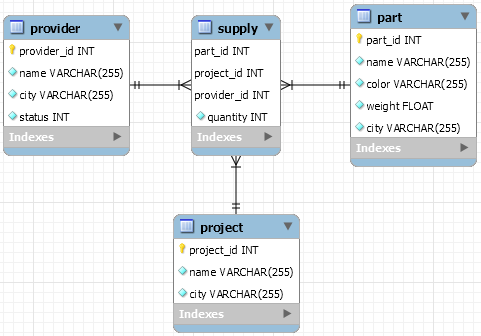
\includegraphics{supply.png}
            \label{fig:supply}
        \end{figure}
    \subsection{Розклад}
        \begin{figure}[H]
            \centering
            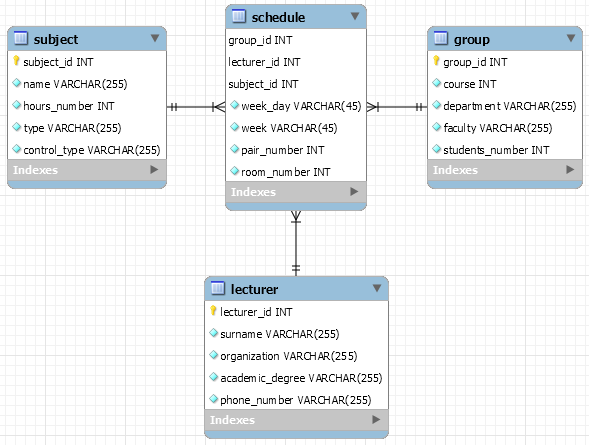
\includegraphics{schedule.png}
            \label{fig:schedule}
        \end{figure}

\end{document}
